\documentclass[12pt]{article}

\usepackage[utf8]{inputenc}
\usepackage[T1]{fontenc}  
\usepackage{hyperref}    
\usepackage{url}   
\usepackage{graphicx}
\usepackage{tabularx}
\usepackage{mathptmx}
\usepackage[romanian]{babel}
\usepackage{indentfirst}
\usepackage{subfig}

\graphicspath{ {./graphics/} }

\hypersetup{
	colorlinks=true,
	linkcolor=blue,
	filecolor=magenta,      
	urlcolor=cyan,
}
\urlstyle{same}

\newcolumntype{C}[1]{>{\centering\arraybackslash}p{#1}}


\title{\textbf{Raport final - Automatic 2D-to-3D image conversion}}

\author{
 	ECHIPĂ: E6
	\\
	 Beldiman Vladislav Student1
	\\
	Grupa 1305A
}

\begin{document}

\noindent\begin{minipage}{0.1\textwidth}
	
\includegraphics[width=1.1cm]{logo_AC.png}
\end{minipage}
\hfill
\begin{minipage}{1\textwidth}\raggedright
	Universitatea Tehnică "Gheorghe Asachi" din Iași\\
	Facultatea de Automatică și Calculatoare\\
	Prelucrarea Imaginilor - Proiect
\end{minipage}

{\let\newpage\relax\maketitle}

\maketitle
\begin{abstract}
Proiectul dat reprezintă o aplicație Windows cu interfață grafică care realizează conversia unei imagini din 2D în 3D cu interacțiune minimă în cadrul acestui proces din partea utilizatorului. Acest lucru e realizat considerând intensitatea fiecărui pixel drept valoarea înălțimii acestuia într-un câmp de înălțimi, iar pe baza acestor valori e construită o plasă poligonală cu fețe triunghiulare (Figura \ref{fig:fig1}).

Triangulația domeniului determinat de pixeli e realizată prin triangulația naivă (Figura \ref{fig:fig2}) care include toate punctele corespunzătoare pixelilor, sau prin aproximare prin înserare lacomă secvențială (Figura \ref{fig:fig3}) cu sau fără aplicarea triangulației Delaunay[1]. Înserarea lacomă va folosi drept măsură de importanță pentru fiecare punct eroarea verticală dintre valoarea câmpului și aproximarea interpolată în acel punct.

Aplicația e scrisă în limbajul de programare C++ cu interfața grafică realizată cu ajutorul setului de instrumente Qt, iar plasa poligonală e sintetizată folosind interfața pentru programarea aplicațiilor OpenGL. Ea permite vizualizarea imaginii încărcate și finale, cât și salvarea imaginii 3D în format STL.

Utilizatorul are opțiunea de a selecta algoritmul de triangulație, selecta eroarea maximă la triangulație (unde e cazul), inversara imaginea finală (răsturnarea valorilor din câmp) și selecta înălțimea dintre valoarea maximă și minimă de gri.

Am constatat faptul că utilizarea unei aproximări prin înserare lacomă fără aplicarea triangulației Delaunay de cele mai multe ori la prezența unui număr mare de triunghiuri care au un unghi sau două extrem de ascuțite, care duce la un număr cu mult mai mare de puncte și triunghiuri în plasa finală, de unde rezultă și un timp mai mare de execuție, cât și, specific pentru aplicația dată, a zonelor care arată ca un burduf de acordeon unde se concentrează multe astfel de triunghiuri.

\textbf{Cuvinte cheie: \color{red} Câmp de înălțimi, Triangulație, Plasă poligonală \color{black}}
\end{abstract}

\begin{figure}[!htb]
	\begin{minipage}{0.32\textwidth}
		\centering
		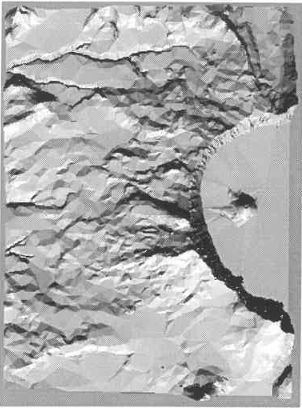
\includegraphics[width=.7\linewidth]{ExempluPlasa.png}
		\caption{Exemplu de plasă poligonală rezultantă. [1]}\label{fig:fig1}
	\end{minipage}\hfill
	\begin{minipage}{0.32\textwidth}
		\centering
		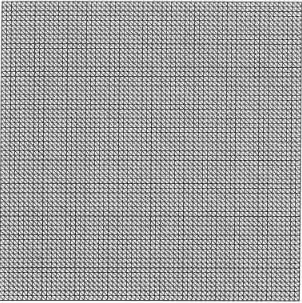
\includegraphics[width=.7\linewidth]{ExempluTriangulatieNaiva.png}
		\caption{Exemplu de triangulație naivă. [1]}\label{fig:fig2}
	\end{minipage}\hfill
	\begin{minipage}{0.32\textwidth}
		\centering
		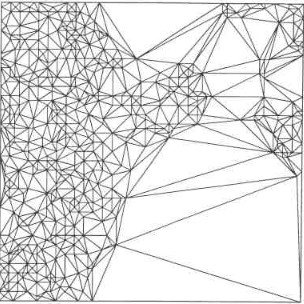
\includegraphics[width=.7\linewidth]{ExempluTriangulatieCuAproximari.png}
		\caption{Exemplu de triangulație care aproximează un câmp de înălțimi. [1]}\label{fig:fig3}
	\end{minipage}
\end{figure}

\section{Introducere}

Această aplicație are diverse utilități, în special deoarece printer-ele 3D au devenit accesibile. Începând cu necesități industriale în dezvoltarea jocurilor video 3D până la crearea litofanelor (fr. lithophanie) pentru decorarea interiorului din confortul biroului de acasă.

În contextul jocurilor 3D, ea poate fi folosită pentru crearea unei plase poligonale dintr-o imagine pentru o entitate, sau generarea terenului pentru joc dintr-o imagine 2D. De exemplu, în figura \ref{fig:fig5} e prezentată generearea unui teren dintr-o imagine generată \href{https://cpetry.github.io/TextureGenerator-Online/}{online} utilizând zgomot perlin.

În plus, ea poate fi utilizată pentru a scoate în evidență anumite detalii dintr-o imagine cu scopul de a îmbunătăți prezentarea, cum ar fi evidențierea unei regiuni de pe o hartă (figura \ref{fig:fig7}) sau crearea unei reprezetări 3D a unei diagrame (figura \ref{fig:fig9}).

Un alt exemplu de utilizare ar fi cel al creării litofanelor care sunt opere gravate realizate din poțelan translucid foarte subțire care poate fi văzut clar doar atunci când e iluminat din spate. Folosind rezultatul aplicației, însă, putem utiliza un printer 3D pentru a crea una folosind un material translucent (figura \ref{fig:fig9}).

\begin{figure}[!htb]
	\begin{minipage}{0.24\textwidth}
		\centering
		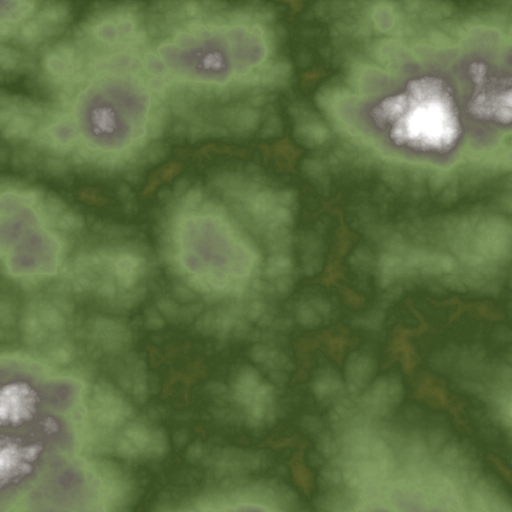
\includegraphics[width=0.95\linewidth]{Teren/TerenImg.png}
		\caption{Imaginea generată cu zgomot perlin.}\label{fig:fig4}
	\end{minipage}\hfill
	\begin{minipage}{0.24\textwidth}
		\centering
		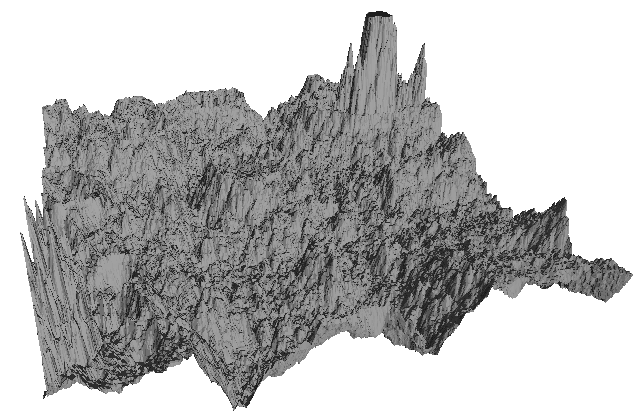
\includegraphics[width=.95\linewidth]{Teren/TerenMesh.png}
		\caption{Terenul generat.}\label{fig:fig5}
	\end{minipage}\hfill
        \begin{minipage}{0.24\textwidth}
		\centering
		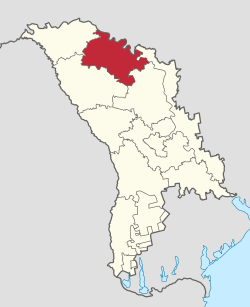
\includegraphics[width=.95\linewidth]{Harta/HartaImg.png}
		\caption{Hartă cu o zonă colorată.}\label{fig:fig6}
	\end{minipage}\hfill
	\begin{minipage}{0.24\textwidth}
		\centering
		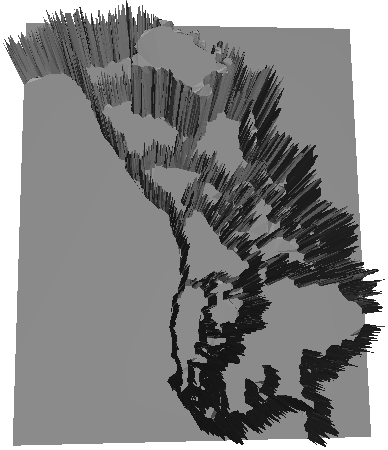
\includegraphics[width=.95\linewidth]{Harta/HartaMesh.png}
		\caption{Evidențierea zonei în 3D.}\label{fig:fig7}
	\end{minipage}\hfill
\end{figure}

\begin{figure}[!htb]
	\begin{minipage}{0.24\textwidth}
		\centering
		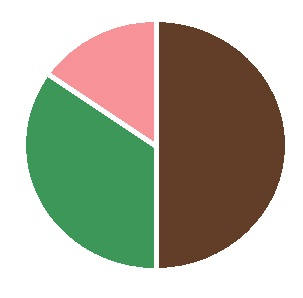
\includegraphics[width=.95\linewidth]{Diagrama/DiagramaImg.jpg}
		\caption{Diagrama circulară.}\label{fig:fig8}
	\end{minipage}\hfill
	\begin{minipage}{0.24\textwidth}
		\centering
		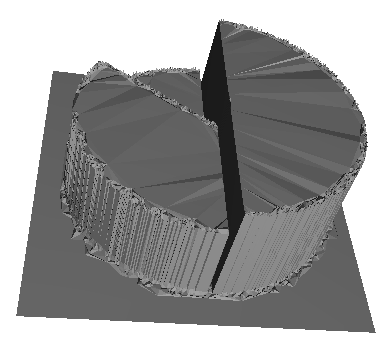
\includegraphics[width=.95\linewidth]{Diagrama/DiagramaMesh.png}
		\caption{Bucățile scoase în evidență conform proporției.}\label{fig:fig9}
	\end{minipage}\hfill
        \begin{minipage}{0.24\textwidth}
		\centering
		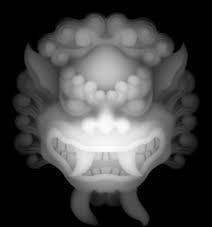
\includegraphics[width=.95\linewidth]{Lithophane/LithophaneImg.jpg}
		\caption{Imaginea pentru litofan.}\label{fig:fig10}
	\end{minipage}\hfill
	\begin{minipage}{0.24\textwidth}
		\centering
		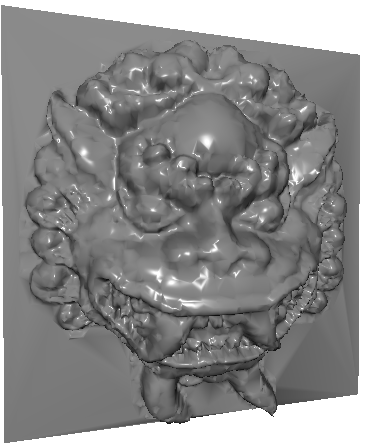
\includegraphics[width=.95\linewidth]{Lithophane/LithophaneMesh.png}
		\caption{Litofanul.}\label{fig:fig11}
	\end{minipage}\hfill
\end{figure}

\section{Metode existente}

Metodele generale existente în literatură au aceeași intrare - o imagine 2D în tonuri de gri (sau una color care e convertită), iar drept ieșire o plasă poligonală stocată într-un anumit format, cum ar fi StL. Ele diferă în primul rând prin algoritmul de triangulație utilizat. De asemenea, ele diferă prin măsuri de importanță (în cazul algoritmilor care realizează aproximări), gradul de optimizare, precum structurile de date utilizate pentru stocarea punctelor și a triunghiurilor și metodele numerice utilizate pentru a reduce erorile de date. În continuare vor fi explorate doar metodele de triangulație, deoarece optimizările nu prezintă scopul principal al acestui proiect, care pot fi găsite în literatură.

Cea mai simplă dintre metode e cea de triangulație naivă[1]. Plasa poligonală rezultantă în urma utilizării acesteea conține câte un vârf pentru fiecare pixel din imaginea inițială care are înălțimea proporțională cu tonul de gri din imagine și câte două triunghiuri pentru fiecare vârf, mai puțin o linie și o coloană. E banal de implementat, e rapidă, deoarece parcurge imaginea și vârfurile câte o singură dată, însă rezultă într-un număr foarte mare de puncte și triunghiuri indiferent de imaginea de la intrare, de exemplu pentru o imagine de doar 512 px x 512 px obținem peste jumătate de milion de triunghiuri.

O metodă care rezultă într-o aproximare a plasei obținute prin algoritmul naiv este cea de inserție lacomă utilizând triangulația Delaunay[1]. În cadrul acestei metode la fiecare pas e adăugat câte un vârf de importanță maximă, de exemplu eroarea locală maximă, sunt adăugate triunghiurile care pot fi create folosind acest și fiecare doi vecini alăturați, după care se verifică dacă proiecția plasei pe planul XOY respectă condiția Delaunay și refăcută, după caz, întorcând latura comună. În plus, dacă măsura de importanță permite acest lucru, e exploatată localitatea schimbărilor care apar în plasă prin recalcularea măsurii doar în punctele care aparțin triunghiurilor incidente vârfului adăugat.

O altă metodă de aproximare e triangulația dependentă de date[1]. Aceasta are la bază triangulația Delaunay, însă, spre deosebire de aceasta, metoda dată nu utilizează doar proiecția pe plan, întorcând latura comună între două triunghiuri dacă nu e respectată condiția Delaunay doar în cazul în care e obținută o eroare globală mai mică.

\textbf{Git repository:} \url{https://github.com/veeyslaw/hfbm}

\section{Descrierea tehnică a soluției}

Datele plasei sunt stocate atât în timpul triangulației, cât și după, după cum urmează: coordonatele vârfurilor într-un vector tridimensional, la care va fi adăugată după finisarea algoritmului date despre culorile și normalele cu scopul de a le sintetiza în QOpenGLWidget, iar în loc de a stoca majoritatea punctelor de mai multe ori, va fi folosit un tablou de indici, câte 3 pentru fiecare triunghi, fiecare din ei reprezentând poziția în tabloul de vârfuri al vârfurilor care îl alcătuiesc, eliminând nevoia de a stoca de două ori punctele fiecărei lature comune din plasă. În plus, OpenGL ne permite să folosim și această reprezentare la tamponarea datelor pentru sintetizare. Indicii apar în ordine trigonometrică, ordine conformă cu standardul StL [2], și cu modul implicit în care detectează OpenGL orientarea triunghiurilor.

Conform standardului StL [2]:
\begin{itemize}
	\item Un fișier StL constă dintr-o listă de date despre fațete;
	\item Orientarea fațetelor e specificată redundant în două moduri - prin direcția normalei și prin ordinea în care sunt specificate vârfurile - trigonometrică;
	\item Fiecare triunghi trebuie să împartă două vârfuri cu fiecare două triunghiuri vecine;
	\item Formatul binar e compus dintr-un antet pe 80 de bytes care nu are nici o semnificație de dată, 4 bytes de tipul unsigned long integer - numărul de fațete în fișier, după care pentru fiecare triunghi sunt adăugate datele: 3 x 4 bytes de tip float care reprezintă vectorul normalei, câte 3 x 4 bytes de tip float pentru toți cei 3 vectori - vârfuri, și 2 bytes de tip unsigned integer care nu vor avea vreo însemnătate în cadrul proiectului.
\end{itemize}

În cadrul algoritmului de triangulație naivă este adăugat câte un vârf pentru fiecare punct din imaginea sursă având ca valoare pe axa Oz valoarea de gri a imaginii. După care, pentru fiecare punct în afară de cele de pe prima coloană și primul rând sunt adăugate câte 2 triunghiuri în tabloul de indici după cum e prezentat în figura \ref{fig:fig12}.

Al doilea algoritm de triangulație implementat este cel de inserție lacomă fără verificarea condiției Delaunay, iar măsura de importanță utilizată e eroarea locală, care reprezintă diferența între aproximația și valoarea din câmpul de înălțimi în acel punct raportată la înălțimea maximă posibilă. În primul rând, sunt adăugate 4 vârfuri corespunzătoare colțurilor imaginii și 2 triunghiuri formate utilizând aceste vârfuri conform algorimului descris la triangulația naivă. Apoi, la fiecare pas e localizat unul din punctele cu eroare maximă, iar dacă eroarea maximă e mai mică decât eroarea maximă admisă de utilizator algoritmul produce plasa poligonală la ieșire, altfel continuă execuția adaugând vârful corespunzător acestui punct în plasă. După adăugarea unui vârf, e localizat triunghiul care îl conține. Proiectând plasa pe planul XOY distingem 3 cazuri: cazul I - punctul proiectat se află în interiorul triunghiului, cazul II - punctul proiectat se află pe frontiera triunghiului și latura pe care e proiectat e împărțită cu un alt triunghi din plasă și cazul III - punctul proiectat se află pe frontiera triunghiului, iar latura pe care e proiectat aparține frontierei plasei. În cazul I (figura \ref{fig:fig12}) adăugăm 3 triunghiuri alcătuite din vârful adăugat și cele 3 perechi distincte de vârfuri ale triunghiului mărginitor. În cazul II (figura \ref{fig:fig13}) sunt înlocuite cele două triunghiuri cu alte 4 alcătuite din vârful adăugat și cele 4 perechi distincte adiacente de vârfuri ale triunghiurilor măriginitoare. În cazul III (figura \ref{fig:fig14}) triunghiul e înlocuit de 2 triunghiuri formate din vârful adăugat și cele 2 perechi distincte de vârfuri ale triunghiului mărginitor care conțin punctul opus laturii pe care e proiectat vârful adăugat.

\begin{figure}[!htb]
	\begin{minipage}{0.24\textwidth}
		\centering
		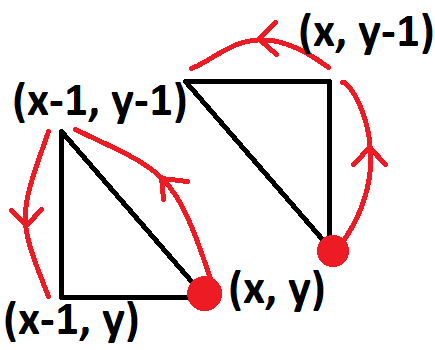
\includegraphics[width=.95\linewidth]{NaivaOrdine.PNG}
		\caption{Inserția în algoritmul naiv.}\label{fig:fig12}
	\end{minipage}\hfill
	\begin{minipage}{0.24\textwidth}
		\centering
		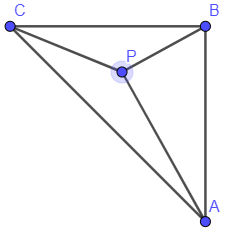
\includegraphics[width=.95\linewidth]{cazi.png}
		\caption{Cazul I.}\label{fig:fig13}
	\end{minipage}\hfill
        \begin{minipage}{0.24\textwidth}
		\centering
		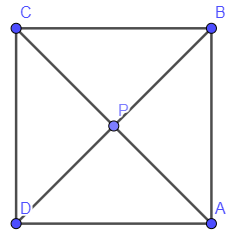
\includegraphics[width=.95\linewidth]{cazii.png}
		\caption{Cazul II.}\label{fig:fig14}
	\end{minipage}\hfill
	\begin{minipage}{0.24\textwidth}
		\centering
		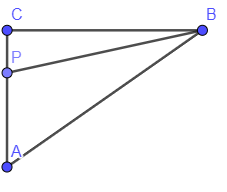
\includegraphics[width=.95\linewidth]{caziii.png}
		\caption{Cazul III.}\label{fig:fig15}
	\end{minipage}\hfill
\end{figure}

Deoarece algoritmul inițial era intolerabil de lent dacă plasa avea mai mult de câteva mii de triunghiuri, am implementat unele optimizări. Prima a fost exploatarea localității modificării erorii locale. Pentru aceasta, în loc de a parcurge toate punctele și dacă nu a fost introdus în plasă, a căuta prin toate triunghiuri pe cel mărginitor și a calcula eroarea, am utilizat un tablou de erori în care e stocată eroarea maximă și punctul corespunzător pentru fiecare triunghi. Astfel, putem exploata faptul că punctul cu eroare maximă dintr-un triunghi se schimbă doar dacă acesta a fost afectat de inserție, iar recalcularea erorilor se face doar pentru aceste triunghiuri iterând prin punctele pătratului care mărginește triunghiul cu verificarea apartenenței interiorului sau a frontierei triunghiului. În plus, a fost redus timpul de căutare al triunghiurilor vecine folosind un tablou în care sunt stocați cei trei vecini ai triunghiului, câte unul pentru fiecare latură.

Al treilea algoritm de triangulație disponibil este inserția lacomă asigurând condiția Delaunay pentru proiecția plasei poligonale pe planul XOY. Detaliile referitoare la inserția lacomă sunt valabile și pentru acest algoritm, atât algoritmul inserției, cât și optimizările. Diferența apare după inserție unde e verificată respectarea condiției Delaunay pentru proiecția plasei. Aici intervine altă optimizare legată de localitatea schimbărilor și anume: dupa inserție, laturile opuse vârfului introdus devin suspecte în ceea ce privește nerespectarea condiției Delaunay, iar, după învârtirea unei laturi, triunghiurile afectate devin suspecte, și, în plus, pentru triunghiurile din urmă trebuie actualizată eroarea maximă din cache. Condiția Delaunay presupune verificarea dacă cercul circumscris unui triunghi conține în interior sau pe frontieră și al patrulea punct (figura \ref{fig:fig16}).

\begin{figure}[!htb]
	\begin{minipage}{0.5\textwidth}
		\centering
		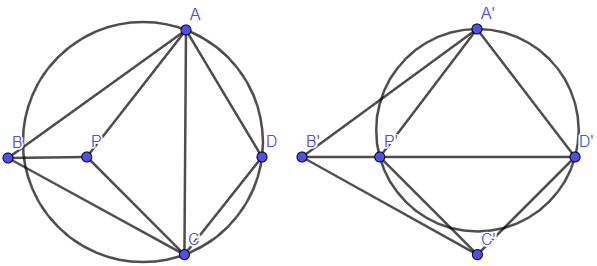
\includegraphics[width=.95\linewidth]{Delaunay.PNG}
		\caption{(a) Condiția Delaunay e încălcată. (b) Triangulația Delaunay refăcută.}\label{fig:fig16}
	\end{minipage}\hfill
\end{figure}

\section{Rezultate experimentale}

Rezultatul esențial observat în timpul experimentelor a fost răspuns la întrebarea apărută în timpul studierii diferitelor metode de triangulație în contextul coversiei a unei imagini 2D în 3D: De ce lucrările studiate care implementează un algoritm de inserție lacomă încep analiza de la triangulația Delaunay, fără a studia un algoritm simplu de triangulație fără verificări suplimentare, precum al doilea algoritm implementat în acest proiect. Răspunsul e prezența triunghiurilor a căror proiecție are un unghi sau două extrem de ascuțite, numite în literatură și triunghiuri "surcea" (eng. sliver triangles). Aceste triunghuri, în spațiu sunt amplasate într-un plan aproape perpendicular pe planul XOY. Acest efect e amplificat atunci când se acumulează într-o zonă, formând o structură asemănătoare cu un burduf de acordeon. Aceste triunghiuri reprezintă o problemă atât din punct de vedere estetic, cât și al aproximării, iar, punctele acestora fiind aproape colineare în planul XOY nu conțin puncte care nu au fost introduse încă în plasă pentru au o îmbunătăți. Aici intervine o proprietate triangulației Delaunay care e maximizarea unghiului minim [3], în urma căreia e ameliorat sau chiar eliminat efectul acestor triunghiuri. În plus, experimentele arată faptul că în urma aplicării triangulației Delaunay plasa rezultantă conține mai puține triunghiuri decât inserția lacomă cu triangulație simplă.

Din rezultatele experimentale poate fi observat faptul că triangulația naivă e cea mai rapidă, însă rezultă într-un număr foarte mare de triunghiuri. Inserția lacomă cu triangulația Delaunay durează cu mult mai mult, însă poate rezulta într-un număr foarte mic, relativ la prima metodă. Iar inserția lacomă cu triangulație simplă durează cel mai mult, ocupă mai mult spațiu decât Delaunay, dar mai puțin decât cea naivă, însă un dezavantaj mare e aproximarea prostă acolo unde apar triunghiuri surcea. Diferențele între algorimul naiv și cel care folosește triangulația Delaunay sunt mai pronunțate cu cât imaginea e mai uniformă (nu conține variații bruște ale intensității).

\begin{figure}[!htb]
	\begin{minipage}{0.24\textwidth}
		\centering
		
\includegraphics[width=.95\linewidth]{Turn/TurnImg.jpg}
		\caption{O imagine (256 px x 256 px).}\label{fig:fig17}
	\end{minipage}\hfill
	\begin{minipage}{0.24\textwidth}
		\centering
		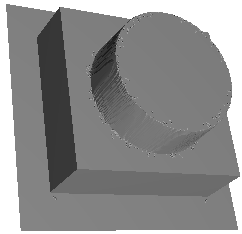
\includegraphics[width=.95\linewidth]{Turn/TurnNaiva.png}
		\caption{Algoritm naiv (0.01 s, 6350.18 KB).}\label{fig:fig18}
	\end{minipage}\hfill
        \begin{minipage}{0.24\textwidth}
		\centering
		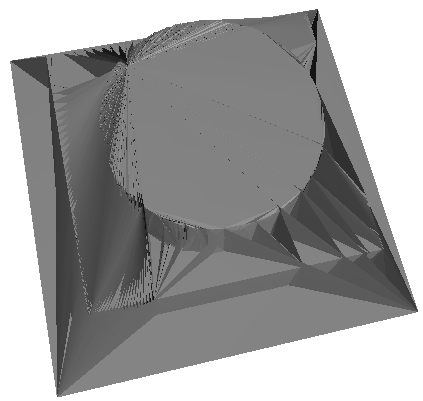
\includegraphics[width=.95\linewidth]{Turn/TurnGreedy.png}
		\caption{Inserție lacomă triangulație simplă 1\% (3.60 s, 394.32 KB).}\label{fig:fig19}
	\end{minipage}\hfill
	\begin{minipage}{0.24\textwidth}
		\centering
		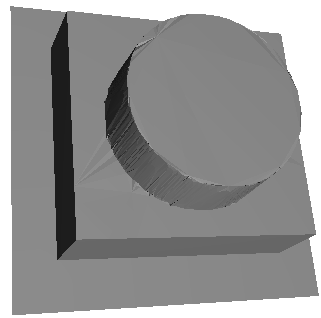
\includegraphics[width=.95\linewidth]{Turn/TurnDelaunay1.png}
		\caption{Inserție lacomă triangulație Delaunay 1\% (1.14 s, 92.27 KB).}\label{fig:fig20}
	\end{minipage}\hfill
\end{figure}

\begin{figure}[!htb]
	\begin{minipage}{0.24\textwidth}
		\centering
		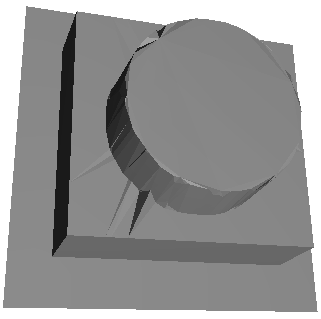
\includegraphics[width=.95\linewidth]{Turn/TurnDelaunay10.png}
		\caption{Inserție lacomă triangulație Delaunay 10\% (1.09 s, 41.39 KB).}\label{fig:fig21}
	\end{minipage}\hfill
        \begin{minipage}{0.24\textwidth}
		\centering
		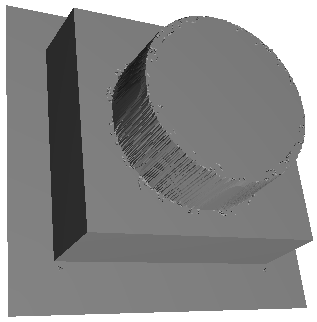
\includegraphics[width=.95\linewidth]{Turn/TurnDelaunay001.png}
		\caption{Inserție lacomă triangulație Delaunay 0.01\% (1.6271 s, 244.61 KB).}\label{fig:fig22}
	\end{minipage}\hfill
        \begin{minipage}{0.24\textwidth}
		\centering
		
\includegraphics[width=.95\linewidth]{Text/TextImg.jpg}
		\caption{Imagine text (573 px x 201 px).}\label{fig:fig23}
	\end{minipage}\hfill
        \begin{minipage}{0.24\textwidth}
		\centering
		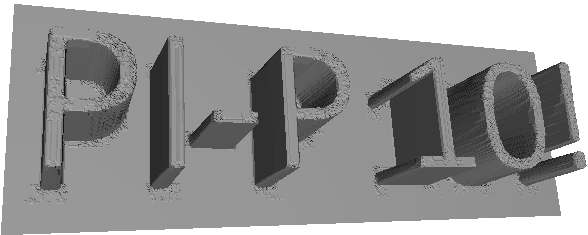
\includegraphics[width=.95\linewidth]{Text/TextNaiv.png}
		\caption{Algoritm naiv (0.02 s, 11172 KB).}\label{fig:fig24}
	\end{minipage}\hfill
\end{figure}

\begin{figure}[!htb]
	\begin{minipage}{0.24\textwidth}
		\centering
		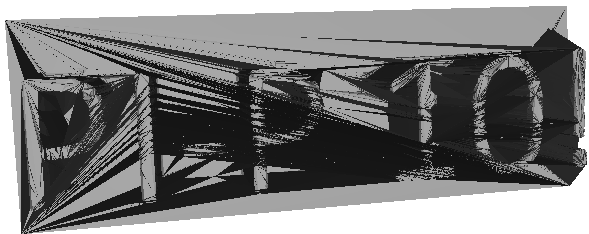
\includegraphics[width=.95\linewidth]{Text/TextGreedy.png}
		\caption{Inserție lacomă triangulație simplă 1\% (17.63 s, 1273.03 KB).}\label{fig:fig25}
	\end{minipage}\hfill
        \begin{minipage}{0.24\textwidth}
		\centering
		
\includegraphics[width=.95\linewidth]{Text/TextDelaunay1.png}
		\caption{Inserție lacomă triangulație Delaunay 1\% (3.37 s, 662.68 KB).}\label{fig:fig26}
	\end{minipage}\hfill
        \begin{minipage}{0.24\textwidth}
		\centering
		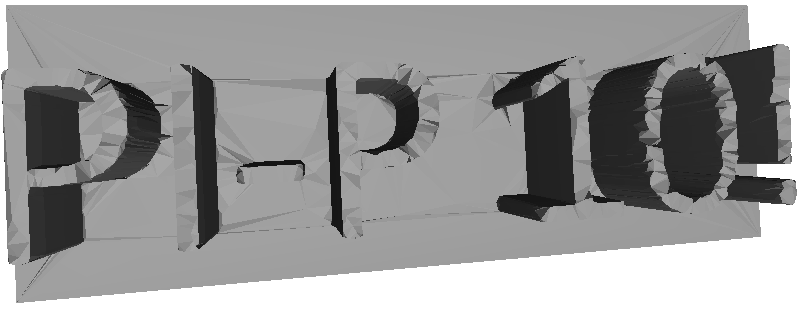
\includegraphics[width=.95\linewidth]{Text/TextDelaunay10.png}
		\caption{Inserție lacomă triangulație Delaunay 10\% (1.84 s, 227.72 KB).}\label{fig:fig27}
	\end{minipage}\hfill
        \begin{minipage}{0.24\textwidth}
		\centering
		
\includegraphics[width=.95\linewidth]{Text/TextDelaunay001.png}
		\caption{Inserție lacomă triangulație Delaunay 0.01\% (11.60 s, 2184.26 KB).}\label{fig:fig28}
	\end{minipage}\hfill
\end{figure}

\begin{figure}[!htb]
	\begin{minipage}{0.24\textwidth}
		\centering
		
\includegraphics[width=.95\linewidth]{Sah/SahImg.png}
		\caption{Imagine pixeli alb-negru organizare tablă de șah. (300 px x 100 px).}\label{fig:fig29}
	\end{minipage}\hfill
        \begin{minipage}{0.24\textwidth}
		\centering
		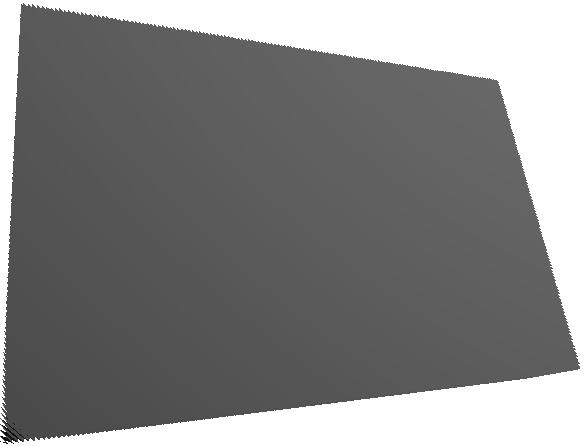
\includegraphics[width=.95\linewidth]{Sah/SahNaiv.png}
		\caption{Algoritm naiv (0.01 s, 5810.73 KB).}\label{fig:fig30}
	\end{minipage}\hfill
        \begin{minipage}{0.24\textwidth}
		\centering
		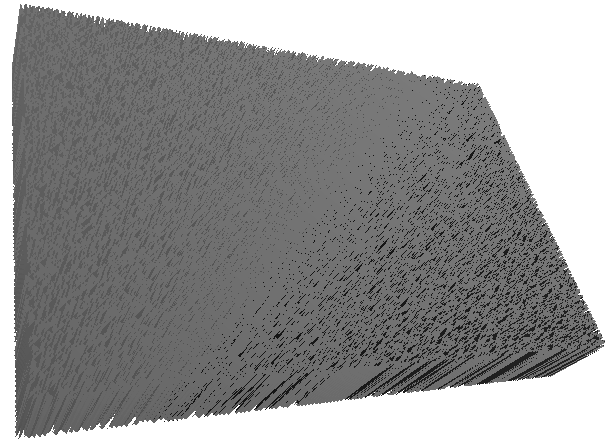
\includegraphics[width=.95\linewidth]{Sah/SahDelaunay001.png}
		\caption{Inserție lacomă triangulație Delaunay 0.01\% (69.69 s, 5810.73 KB).}\label{fig:fig31}
	\end{minipage}\hfill
        \begin{minipage}{0.24\textwidth}
		\centering
		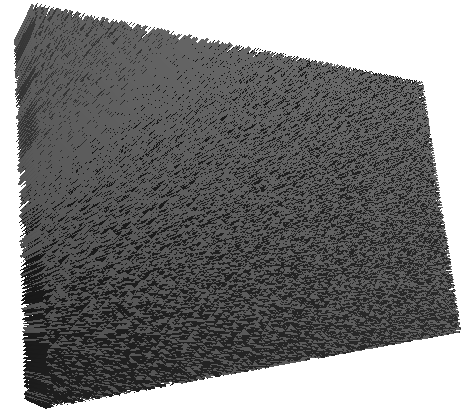
\includegraphics[width=.95\linewidth]{Sah/SahDelaunay50.png}
		\caption{Inserție lacomă triangulație Delaunay 50\% (70.478 s, 5810.73 KB).}\label{fig:fig32}
	\end{minipage}\hfill
\end{figure}

\newpage
\section{Concluzii}

Principalele concluzii care pot fi extrase sunt: dacă e utilizat un algoritm de inserție lacomă, la triangulație trebuie tratate triunghiurile surcea utilizând, de exemplu triangulația Delaunay. Numărul de triunghiuri mai mic rezultat în urma algoritmului cu triangulația Delaunay mărește costul temporal. Algoritmul cu triangulația Delaunay e foarte util atunci când imaginea are multe zone în care intensitațile variază sub eroarea maximă admisă.

Posibile direcții de dezvoltare viitoare ar fi: creșterea gradului de optimizare al algoritmului de inserție lacomă cu triangulație Delaunay. Implementarea algoritmului dependent de date pentru al compara cu celelalte la care ar trebui atrasă atenție deosebită la cum afectează triunghiurle surcea rezultatul, deoarece acesta nu realizează o triangulație Delaunay pură. Dezvoltarea componentei de vizualizare a plasei poligonale încorporate. Adăugarea culorii la imaginile generate, folosind ultimul câmp de 2 bytes care nu e utilizat oficial, însă e utilizat de unele produse software cu acest scop, și implementarea unui algoritm de interpolare a culorii în elementul de vizualizare pentru a le reprezenta.

\section*{Referințe}

\medskip

[1] \href{http://reports-archive.adm.cs.cmu.edu/anon/anon/home/ftp/1995/CMU-CS-95-181.pdf} {Garland M. and Heckbert P. S. (1995) Fast Polygonal Approximation of Terrains and Height Fields. (CMU-CS-95-181)}

[2] \href{https://www.fabbers.com/tech/STL_Format#Sct_binary} {Marshall Burns. Automated Fabrication
Improving Productivity in Manufacturing.}

[3] \href{http://www.comp.nus.edu.sg/~tants/Paper/mma.pdf} {H. Edelsbrunner, T. Seng Tan and R. Waupotitsch. An O(n log n) time algorithm for the minmax angle triangulation.}

\end{document}